% =============================================================================
% Section 3: Data
% Specification: config/raw_inputs_manifest.yml, docs/sources.md, docs/methodology.md,
%   scripts/10_build_themes.R, scripts/12-15, scripts/98_pull_comtrade_energy_dyads.R,
%   R/utils/country.R, R/categories/trade/trade_core.R, data/reference/energy_hs6_master.csv.
% Numbers: paper/results/method.json, hs6_crosswalk.json, bilateral.json, coalition.json
%   (final rerun of 12 October 2026). Release rule, harmonisation, vintages and the years of
%   each source: Online Appendix oa:data (sections/oa_data.tex).
% =============================================================================

\section{Data}\label{sec:data}

The indices combine public statistical releases, licensed commercial datasets and a few
project-authored tables. Appendix~\ref{app:sources} lists every source with its publisher,
coverage and release, Appendix~\ref{app:variables} every variable built from it, and Online
Appendix~\ref{oa:data} the rule that selects a release, the harmonisation of economy names and
the years each source covers.

% -----------------------------------------------------------------------------
\subsection{Sources by pillar}\label{subsec:data_families}

Table~\ref{tab:data_families} groups the sources by what they measure. Most report economies,
but some report the world (commodity prices, demand projections, technology readiness) or a few
regions (manufacturing capacity, relative equipment costs); such a variable shifts a pair's level
without ranking economies within it. Coverage ranges from about two hundred economies for trade
and energy statistics to a few dozen for levelised costs, a gap that the missing-data rules of
Section~\ref{subsec:norm_missing} bridge.

\begin{table}[tbp]
\centering
\begin{threeparttable}
\caption{Source families, levels of observation and what they feed}
\label{tab:data_families}
\footnotesize
\begin{tabularx}{\textwidth}{@{}>{\raggedright\arraybackslash}p{2.3cm}
  >{\raggedright\arraybackslash}X >{\raggedright\arraybackslash}p{2.0cm}
  >{\raggedright\arraybackslash}p{4.2cm}@{}}
\toprule
Family & Sources & Level & Feeds\\
\midrule
Energy statistics & EI Statistical Review 2026; EIA International Energy Statistics (fuel
  production EI does not report) & Economy & ES: energy access, consumption, energy imports,
  reserves (fossil), production (minerals). EO: energy access, production\\[2pt]
Reserves and uranium & USGS Mineral Commodity Summaries 2026; OECD-NEA/IAEA Red Book (Uranium
  2026); EI proved reserves & Economy & ES: reserves, production (uranium). EO: production
  (uranium). Coalition supplier test\\[2pt]
Trade & UN Comtrade all-reporter dyads (2020, 2024) and their World totals; Atlas of Economic
  Complexity (HS92); Comtrade critical-minerals extracts & Economy; dyad & ES: trade, minerals
  trade. EO: trade. Friendshore, Partnership Opportunity, network edges\\[2pt]
Minerals and manufacturing & IEA Critical Minerals Dataset 2026; IEA ETP 2024 capacity shares;
  IEA EV regional data & Economy; 5--6 regions & ES and EO: foreign dependency, production;
  mineral demand weights\\[2pt]
Demand and technology & IEA WEO 2025; IEA Global EV Outlook 2026; BNEF New Energy Outlook 2024
  and Supply Chains 2025; BCG market sizing; IEA Clean Energy Technology Guide & World; region;
  United States & ES: consumption. EO: consumption, technology demand, technological
  readiness\\[2pt]
Costs and prices & BNEF LCOE; IEA relative costs; ILOSTAT earnings; IMF lending rates, producer
  prices and commodity prices & Economy; region; world & ES: energy prices. EO: cost
  competitiveness, energy prices\\[2pt]
Potential and investment & Global Solar and Wind Atlases; geothermal potentials; Clean
  Investment Monitor & Economy & ES: reserves (downstream). ES and EO: investment\\[2pt]
Policy & IEA Policies and Measures; Climate Action Tracker; IPCC lifecycle emissions; GTA NIPO
  (robustness only) & Economy; technology & Policy index; technology weight of the SI\\[2pt]
Bilateral and alignment & IMF Direct Investment Positions; CM-FDI projects; WDI; Doing Business;
  OECD CRS; UNGA ideal points; agreement memberships & Dyad; economy & PSI components; blocs,
  coalition, network demand and caps\\
\bottomrule
\end{tabularx}
\begin{tablenotes}[flushleft]\footnotesize
\item \textit{Notes:} ES = Energy Security; EO = Economic Opportunity; SI = Strategic Index;
PSI = Partnership Strength Index. A source reported for a region or for the world is copied to
the economies it covers by the theme that reads it. Appendix~\ref{app:sources} gives publishers,
coverage and releases; Appendix~\ref{app:variables} the variables.
\end{tablenotes}
\end{threeparttable}
\end{table}

\paragraph{Energy security.} The Statistical Review of World Energy \citep{ei2026statistical},
2026 edition with data to 2025, supplies consumption per capita and its growth, the fuel balances
behind energy imports, mineral production and the proved reserves of oil, gas and coal, which the
Review holds at end-2020. Fossil production that the Review counts only in a regional residual
is taken from the U.S. Energy Information Administration \citep{eia2026international}, in the
Review's units and paired with consumption of the same year, as an observation (Estonian coal,
where the Review counts oil shale, stays missing). Critical-mineral reserves at end-2025 (cobalt,
lithium, graphite, rare earths, copper, manganese, nickel, zinc and the platinum-group metals)
come from the USGS Mineral Commodity Summaries 2026 \citep{usgs2026mcs}, with the erratum that
puts Brazil's rare-earth reserves at 11~Mt; holders listed without a figure (``NA'', ``W'',
``s'') count as zero in the technology roll-ups. Nuclear Upstream is scored on the OECD-NEA/IAEA
Red Book \citep{oecdnea2026uranium}: identified recoverable resources below USD 260/kgU at
1 January 2025 (59 economies) and mine production in 2019--2024 (18 producers in 2024), with
economies absent from the tables recorded as zero. The IEA Critical Minerals Dataset
\citep{iea2026cmdata} provides mining (Upstream) and refining (Midstream) supply by economy and
the clean-technology demand that weights each mineral within a technology. Midstream capacity
shares come from IEA Energy Technology Perspectives \citep{iea2024etp}, taken over the world total
including the source's ``Other'' row. Its 2035 announced-capacity shares are regional for
Europe, so every EU member carries the EU's share (0.15 in Wind, 0.11 in Batteries, 0.24 in Green
Hydrogen and 0.00 in Solar Midstream) in the foreign-dependency and market-share variables, which
therefore do not separate the members. Commodity prices (IMF Primary Commodity Price System, \citealp{imf2026pcps}),
clean-technology investment (Clean Investment Monitor, \citealp{cim2026}) and three geospatial
resource-potential datasets complete the pillar.

\paragraph{Economic opportunity.} Export capability rests on the Growth Lab's reconciled HS92 data
underlying the Atlas of Economic Complexity \citep{growthlab2019trade,hausmann2014atlas}, newest
year 2023, and on the 2024 Comtrade exports of Section~\ref{subsec:data_trade}. Demand comes from
the IEA World Energy Outlook 2025 and Global EV Outlook 2026 \citep{iea2025weo,iea2026gevo},
BloombergNEF's New Energy Outlook 2024 \citep{bnef2024neo} and Supply Chains 2025 workbook, and a
Boston Consulting Group sizing of the U.S. addressable market. Costs combine BloombergNEF levelised
costs, IEA relative equipment costs, ILOSTAT earnings, IMF lending rates (placeholder zero
readings dropped) and producer prices. The BloombergNEF and BCG inputs are licensed, which
prevents a fully public replication of this pillar.

\paragraph{Technology readiness by stage.} The IEA Clean Energy Technology Guide
\citep{iea2026cleantechguide} rates technology designs and components on an eleven-point
readiness scale. Ordered rules assign each item to a technology and a stage or classify it as out
of scope: 253 of the 634 items of the 2026 release map to a headline technology. A cell's
readiness is computed from the items of its own stage; a stage without an item, 10 of the 33
cells, takes the technology-wide value. Readiness has no country dimension and is copied to every
economy as an observation.

\paragraph{Policy.} The Policy index combines the IEA Policies and Measures database
\citep{iea2026pams} (export of 22 January 2026), weight 3, and the Climate Action Tracker ratings
\citep{cat2026ratings} (39 countries and the EU, whose rating its unrated members take), weight 2.
IEA PAMS is required and CAT added where it rates the country: 215 economies are scored, 65 on
both and 150 on IEA PAMS alone (Section~\ref{sec:strategic}). The New Industrial Policy
Observatory of Global Trade Alert \citep{gta2026nipo} enters only a robustness variant
(Section~\ref{sec:robustness}). The technology weight of the Strategic Index uses the IPCC
lifecycle-emission medians \citep{schlomer2014annex}.

\paragraph{Bilateral, alignment and coalition inputs.} Outward direct-investment positions come
from the IMF Direct Investment Positions dataset. Positions with 16 conduit financial centres,
the ten pass-through economies identified by \citet{damgaard2024real} and six offshore centres
(Appendix~\ref{app:variables}), are treated as unobserved on either side of the dyad. In battery, electric-vehicle, solar and wind manufacturing, the investment tie and the
Chinese-parent exposure of Friendshore come instead from the Cleantech Manufacturing FDI dataset
\citep{bandara2026cmfdi}, of whose 1,042 cross-border projects 905 qualify. Development potential
uses the World Development Indicators \citep{worldbank2026wdi}, the 2019 Doing Business scores
\citep{worldbank2020doing,worldbank2021discontinue} and OECD aid data. Geopolitical alignment
uses the all-votes UN General Assembly ideal points of \citet{bailey2017estimating} (Dataverse
V39, \citealp{voeten2009unga}), averaged over sessions 74--78 (2019--2023), and coalition
membership a project-authored list of U.S. free-trade agreements, IPEF, the Minerals Security
Partnership, the G7 and NATO compiled from the official lists (Section~\ref{sec:coalition}).

% -----------------------------------------------------------------------------
\subsection{The HS6 product crosswalk}\label{subsec:data_crosswalk}

Trade enters through baskets of six-digit Harmonized System (HS6) products, one per
technology--stage pair, defined in one version-controlled table
(\texttt{data/reference/energy\_hs6\_master.csv}) from which every trade and bilateral file is
generated. With $H_{ts}$ the codes in the basket of $(t,s)$ and $x_{ih}$ economy $i$'s exports of
product $h$, basket exports are
\begin{equation}\label{eq:data_basket}
  X_{its}=\sum_{h\in H_{ts}}x_{ih},
\end{equation}
and imports, world totals and bilateral flows are aggregated in the same way. Ores,
concentrates, slag and scrap are Upstream, processed materials and components Midstream;
Downstream activity is not a traded-goods stage.

\paragraph{The basket review.} In October 2026 every code was tested for dominant use: it stays
in a technology's basket only if that technology is a main use of the product. Ninety-two basket
rows touching 69 codes failed (47 codes left every basket); each stays in the master with its
reason. The crosswalk now holds 259 codes in 415 basket rows (298 in 490 before): 242 of the
current nomenclature and 17 legacy codes that bridge the HS92 Atlas panels. The exclusions carried
92 percent of the pre-review coal Midstream basket's trade, 69 percent of gas Midstream and 89
percent of batteries Upstream, whose copper ores now belong to the grid
(Table~\ref{tab:hs6_counts}). Electric Grid Upstream held only electrical energy (HS 2716.00),
which made net power exporters the grid's leading suppliers; it now holds seven copper and
aluminium inputs, from ores and bauxite to cathodes and unwrought aluminium, so electricity is
outside every basket. Switching and routing apparatus (HS 8517.62), 32 percent of the pre-review
grid Midstream basket, is telecommunication equipment and left it.

\paragraph{Upstream baskets.} Five Upstream baskets are new: Electric Vehicles (the battery-mineral
ores and the rare earths of permanent magnets), Wind (rare earths), Nuclear (uranium ores and
natural uranium compounds, the heading of most yellowcake, moved from Midstream), Solar (silicon
metal) and Semiconductors (gallium, germanium and indium, carried for description only). The four
that are scored trade USD 3.0 billion (wind) to 21.3 billion (electric vehicles) in 2024. With
them, 18 of the 22 scored Upstream and Midstream pairs have a basket; only Geothermal and Green
Hydrogen have none.

\paragraph{A many-to-many mapping.} The baskets do not partition the product space: 105 codes
(41 percent) belong to more than one basket, 63 to two, 33 to three and 9, the transformer,
switchgear and cable headings, to four, since a power cable is an input to every technology that
connects to the grid. Technology totals are therefore not additive, and the trade variables of
technologies that share codes are mechanically correlated.

\begin{figure}[tbp]
  \centering
  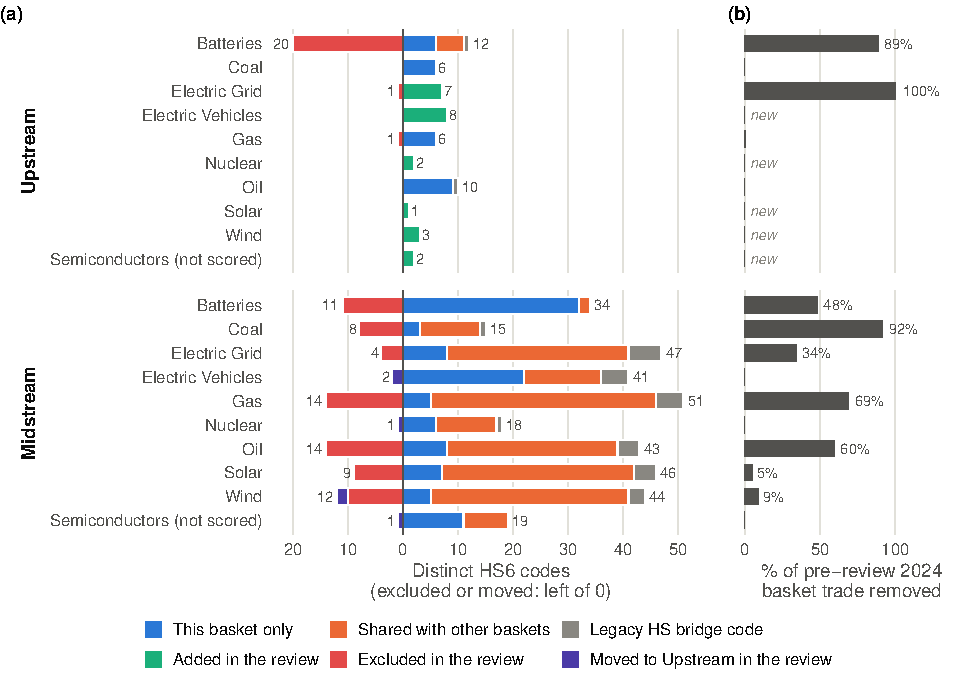
\includegraphics[width=\textwidth]{fig_hs6_crosswalk}
  \caption{The HS6 baskets after the October 2026 review. Panel (a): distinct HS6 codes in each
  technology--stage basket, split into codes of that basket only, current codes shared with at
  least one other basket (the many-to-many part of the mapping), legacy HS bridge codes, and codes
  added by the review (codes moved from a technology's midstream basket count as added to its
  upstream basket); left of zero, the codes the review excluded from the basket and the codes it
  moved to the upstream stage. Panel (b): share of the pre-review basket's 2024 trade value carried
  by the excluded codes; ``new'' marks a basket the review created. Trade is the reconciled
  all-reporter Comtrade matrix (the importer's declaration, else the exporter's declaration
  $\times1.06$), summed over exporter--importer pairs; a code in several baskets counts in each.
  Green hydrogen, geothermal and the downstream stage have no basket; semiconductors are carried
  in the master but not scored. Source: \texttt{data/reference/energy\_hs6\_master.csv},
  \texttt{data/raw/comtrade\_energy\_dyads\_all.csv}; \texttt{scripts/paper/fig\_hs6\_crosswalk.R}.}
  \label{fig:hs6_crosswalk}
\end{figure}

% Generated by scripts/paper/fig_hs6_crosswalk.R; do not edit by hand.
\begin{table}[tbp]
\centering
\begin{threeparttable}
\caption{HS6 baskets by technology and stage after the October 2026 basket review}
\label{tab:hs6_counts}
\footnotesize
\setlength{\tabcolsep}{3.5pt}
\begin{tabular}{@{}llrrrrrrrrr@{}}
\toprule
 & & \multicolumn{4}{c}{Codes in the basket} & \multicolumn{3}{c}{Review} & \multicolumn{2}{c}{Basket trade, 2024} \\
\cmidrule(lr){3-6}\cmidrule(lr){7-9}\cmidrule(l){10-11}
Technology & Stage & All & Legacy & Shared & Sub-sectors & Added & Moved & Excluded & USD bn & \% removed\\
\midrule
Batteries & Upstream & 12 & 1 & 5 & 2 & 0 & 0 & 20 & 21.2 & 88.8\\
 & Midstream & 34 & 0 & 2 & 9 & 0 & 0 & 11 & 202.7 & 48.4\\
Coal & Upstream & 6 & 0 & 0 & 2 & 0 & 0 & 0 & 192.5 & 0.0\\
 & Midstream & 15 & 1 & 12 & 3 & 0 & 0 & 8 & 20.5 & 91.9\\
Electric Grid & Upstream & 7 & 0 & 0 & 3 & 7 & 0 & 1 & 321.0 & 100.0\\
 & Midstream & 47 & 6 & 36 & 12 & 0 & 0 & 4 & 449.6 & 34.3\\
Electric Vehicles & Upstream & 8 & 0 & 8 & 8 & 8 & 0 & 0 & 21.3 & new\\
 & Midstream & 41 & 5 & 17 & 7 & 0 & 2 & 0 & 1,003.2 & 0.0\\
Gas & Upstream & 6 & 0 & 0 & 4 & 0 & 0 & 1 & 445.3 & 0.4\\
 & Midstream & 51 & 5 & 46 & 2 & 0 & 0 & 14 & 151.6 & 69.1\\
Nuclear & Upstream & 2 & 0 & 0 & 2 & 2 & 0 & 0 & 11.4 & new\\
 & Midstream & 18 & 1 & 12 & 3 & 0 & 1 & 0 & 24.6 & 0.0\\
Oil & Upstream & 10 & 1 & 0 & 5 & 0 & 0 & 0 & 2,211.0 & 0.0\\
 & Midstream & 43 & 4 & 35 & 7 & 0 & 0 & 14 & 127.1 & 59.8\\
Solar & Upstream & 1 & 0 & 0 & 1 & 1 & 0 & 0 & 3.8 & new\\
 & Midstream & 46 & 4 & 38 & 9 & 0 & 0 & 9 & 711.5 & 5.5\\
Wind & Upstream & 3 & 0 & 3 & 3 & 3 & 0 & 0 & 3.0 & new\\
 & Midstream & 44 & 3 & 39 & 8 & 0 & 2 & 10 & 409.5 & 9.4\\
Semiconductors\tnote{a} & Upstream & 2 & 1 & 0 & 1 & 2 & 0 & 0 & 1.1 & new\\
 & Midstream & 19 & 0 & 8 & 8 & 0 & 1 & 0 & 1,348.1 & 0.0\\
\midrule
Distinct codes & & 259 & 17 & 105 & 92 & 20 & 4 & 69 & & \\
\bottomrule
\end{tabular}
\begin{tablenotes}[flushleft]\footnotesize
\item \textit{Notes:} Distinct HS6 codes in each technology--stage basket of \texttt{data/reference/energy\_hs6\_master.csv} after the review. ``Legacy'' codes are bridge codes of older HS revisions whose successors are all in the basket; ``Shared'' counts the codes that also belong to at least one other basket. ``Excluded'' counts the codes the review removed from the basket because the technology is not a dominant use of the product, and ``Added'' the codes it added (the copper and aluminium inputs that replace electrical energy, HS 2716.00, in electric-grid Upstream, and the Upstream baskets of electric vehicles, solar, wind, nuclear and semiconductors, which had none); ``Moved'' counts the codes it moved from a technology's Midstream to its Upstream basket (rare-earth compounds and metals, natural uranium compounds, unwrought gallium, germanium and indium), which count as added there, since a code sits in one stage of a technology; the rows stay in the master with the reason. Basket trade is the 2024 value in the reconciled all-reporter Comtrade matrix (the importer's declaration, else the exporter's mirror declaration $\times$ 1.06), summed over exporter--importer pairs; ``\% removed'' is the share of the pre-review basket's value carried by the excluded codes (moved codes are not removals; ``new'' marks a basket the review created). A code in several baskets counts in each, so neither codes nor trade values add across rows. Green hydrogen, geothermal and the Downstream stage have no basket.
\item[a] Carried in the master; not a scored technology.
\end{tablenotes}
\end{threeparttable}
\end{table}


% -----------------------------------------------------------------------------
\subsection{Bilateral trade and the trade themes}\label{subsec:data_trade}

Bilateral flows come from an all-reporter pull of UN Comtrade \citep{uncomtrade} for the
endpoint years 2020 and 2024: 173 economies report in at least one year (168 in 2020; 142 for
exports and 143 for imports in 2024), and 208 appear as reporter or partner. Comtrade records
Taiwan as ``Other Asia, n.e.s.'' (partner code S19), which is mapped to Taiwan's own code. Let
$M^{\mathrm{rep}}_{ji,h}$ be importer $j$'s declared imports of product $h$ from $i$ and
$X^{\mathrm{rep}}_{ij,h}$ exporter $i$'s declared exports to $j$. The flow in a cell is
\begin{equation}\label{eq:data_mirror}
  F_{ij,ts}=
  \begin{cases}
    \sum_{h\in H_{ts}}M^{\mathrm{rep}}_{ji,h} & \text{if $j$ reports imports in the cell that year},\\
    1.06\sum_{h\in H_{ts}}X^{\mathrm{rep}}_{ij,h} & \text{otherwise, if $i$ reports exports to $j$},
  \end{cases}
\end{equation}
and unobserved otherwise; 1.06 is the IMF's conventional ratio of CIF import to FOB export values.
Of the 701,214 exporter--importer--technology--stage cells observed in 2024, 22 percent are
mirror values, but only 13 percent of the cells with positive trade and 4 percent of the value,
because large traders report. Thirty importers that reported in 2020 did not in 2024, among them
Russia, Iran, the United Arab Emirates and Viet Nam, and 65 of the 208 importers enter the 2024
matrix only through their partners' declarations, which omits their imports from exporters that
do not report either.

The country-level trade themes read a file of exports and imports by reporter and code rebuilt
from the World rows of the same pull: 142 exporting and 143 importing reporters in 2024 and every
current-nomenclature basket code, including Qatar's exports of liquefied natural gas (USD 56.9
billion), which the earlier extract omitted. Hong Kong is left out of the Comtrade export measures
(export size, revealed comparative advantage \citep{balassa1965trade} and export concentration)
because its exports are mostly re-exports that the producers' own exports already count; it keeps
its Atlas-based variables, and the bilateral matrix is not filtered. The export-concentration
index is ranked across the cells of the eleven headline technologies only. Critical-minerals
trade uses separate 2024 Comtrade extracts (130 import and 128 export reporters); the 2025
extracts, with three reporters, fall below the coverage floor of the release rule (Online
Appendix~\ref{oa:data}).

% -----------------------------------------------------------------------------
\subsection{Economies, coverage and rankability}\label{subsec:data_countries}

Every economy name in every source is mapped to one canonical name per ISO3 code before anything
is ranked, and world, regional, residual and historical aggregates are dropped. The headline
pillars then cover 219 economies, each with its own ISO3 code, of which 195 are sovereign states
(the 193 members of the United Nations, Kosovo and Taiwan) and 24 are territories, special
administrative regions or the West Bank and Gaza; the same 219 economies (195 sovereign states and
24 territories) have an $\EO$ score, so the two pillars share one universe. Taiwan, which the
World Bank's country table does not list, is carried as an economy throughout, including the trade
themes and the bilateral matrix; it has an $\ES$ value in 28 headline cells and an $\EO$ value in
33. The pillars score 6,232 $\ES$ and 7,131 $\EO$ country--technology--stage cells in 30 and 33
headline pairs. In the alignment data the 193 economies that vote in the General Assembly have an
ideal point; the other economies are treated as Section~\ref{sec:coalition} describes.

The grids span almost the whole universe at every stage, but their width is set by the most
widely distributed theme of each pair. Figure~\ref{fig:method_coverage} separates economies scored
from economies with country-specific data. In $\ES$ the two differ only upstream, where a
commodity-price series copied to every economy sets the grid: by 4 economies in Electric Vehicles
to 38 in Coal, and not at all in Nuclear once absence from the uranium registers is recorded as
zero. In $\EO$ the gap is largest in Electric Grid downstream (143 of 213 economies with
country-specific data). Territories rest more heavily on imputation (mean imputed weight 0.48 of a
territory's $\ES$ cell against 0.29 for a sovereign state; 0.67 against 0.40 in $\EO$).

\begin{figure}[tbp]
  \centering
  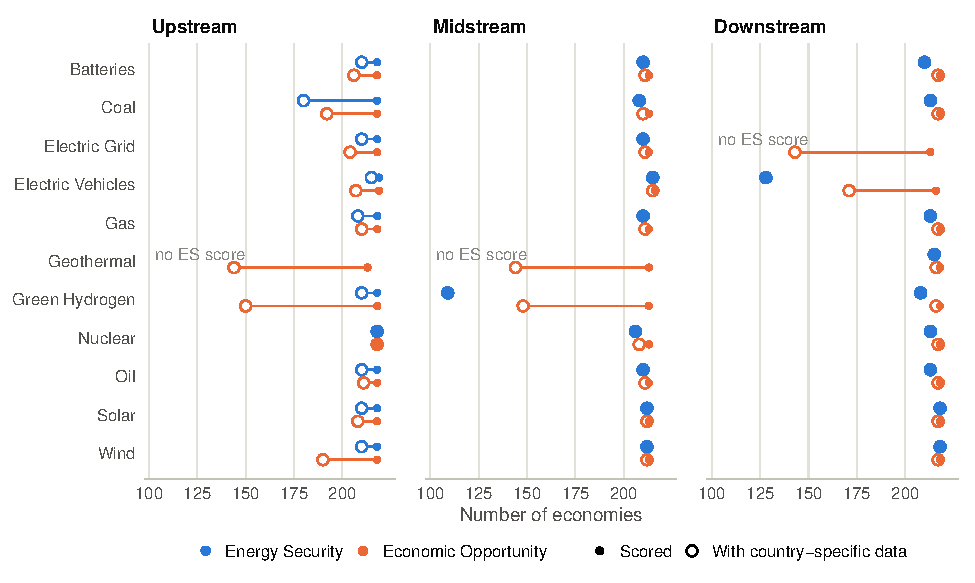
\includegraphics[width=\textwidth]{method_coverage}
  \caption{Economies scored and economies with country-specific data, by technology--stage pair.
  Filled dots: the number of economies with a pillar value in the pair. Hollow circles: the
  number of those economies for which at least one positively weighted, non-imputed component is
  country-specific, that is, takes at least two distinct observed values across the economies of
  the pair. World-level series copied to every economy, such as commodity-price volatility, world
  export concentration and technology readiness, do not count as country-specific. The segment
  between the two marks is the number of economies whose value rests only on imputed components
  and world-level series; where the two counts coincide the marks appear as a ringed dot. ``No ES
  score'' marks the pairs without an $\ES$ value. Every pair has status ok (no pair is constant
  or unscored). The axis starts at 100 economies. Sample: the eleven headline technologies.
  Source: variable contributions and pillar diagnostics in
  \texttt{data/processed/outputs/index\_outputs.rds}; \texttt{scripts/paper/fig\_method.R}.}
  \label{fig:method_coverage}
\end{figure}

Because coverage is uneven, every cell is scored but not every cell is ranked: a cell enters a
ranking, a top-$N$ list, the Strategic Index or the partner rankings only if the economy is
sovereign and at most half of its index weight rests on imputed components
(Section~\ref{subsec:norm_rankability}). The rule keeps 4,163 of the 6,232 $\ES$ cells and 4,301
of the 7,131 $\EO$ cells. Each component is taken at the latest year its source reports, so a cell
can combine observations from 2023 to 2025 with projections to 2035 and, in $\ES$ reserves,
end-2020 fossil stocks (Section~\ref{subsec:norm_latest}).
